\documentclass{article}
\usepackage[utf8]{inputenc}
\usepackage{geometry}                		% See geometry.pdf to learn the layout options. There are lots.
%\usepackage[parfill]{parskip}    		% Activate to begin paragraphs with an empty line rather than an indent
\usepackage{graphicx}				% Use pdf, png, jpg, or eps§ with pdflatex; use eps in DVI mode
								% TeX will automatically convert eps --> pdf in pdflatex		
\usepackage{amssymb}
\usepackage{amsmath}
\usepackage{gensymb} 
\usepackage{cite}
\usepackage{multirow}
\usepackage{wrapfig}
\usepackage{wasysym }
\usepackage{tabu}
\usepackage{array}
\usepackage{booktabs}
\usepackage{graphics}
\usepackage{comment}
\usepackage{caption}
\usepackage{subcaption}
\usepackage{footnote}
\usepackage{threeparttable}
\usepackage{pdflscape}
\usepackage{float}
\usepackage{setspace}
\usepackage{bigstrut}
\usepackage{rotating}
\usepackage{longtable}
\usepackage{indentfirst}
\usepackage{hyperref}
\usepackage{makecell}

\hypersetup
{
  bookmarks=true,         % show bookmarks 
  unicode=false,          % non-Latin characters in Acrobat's bookmarks
  pdftoolbar=true,        % show Acrobat's toolbar?
  pdfmenubar=true,        % show Acrobat's menu?
  pdffitwindow=false,     % window fit to page when opened
  pdfstartview={FitH},    % fits the width of the page to the window
  pdftitle={My title},    % title
  pdfauthor={Author},     % author
  pdfsubject={Subject},   % subject of the document
  pdfcreator={Creator},   % creator of the document
  pdfproducer={Producer}, % producer of the document
  pdfkeywords={keywords}, % list of keywords
  pdfnewwindow=true,      % links in new window
  colorlinks=true,       % false: boxed links; true: colored links
  linkcolor=blue,          % color of internal links
  citecolor=blue,        % color of links to bibliography
  filecolor=magenta,      % color of file links
  urlcolor=blue          % color of external links
}


\usepackage{multicol}
\usepackage{framed}
\usepackage{tcolorbox}
\usepackage[natbibapa]{apacite}
\doublespacing

\title{Logistic Curve Models of $\mathrm{CO_{2}}$ Accumulation}
\author{David Levinson}
\date{July 2020}

\begin{document}

\maketitle

\section*{Abstract}

This article explores the use of logistic-shaped diffusion curves (S-Curves) to predict the accumulation of atmospheric $\mathrm{CO_{2}}$.  The research question here is whether forecasts using logistic curves are stable, that is, do they predict consistently over time with different amounts of data?  Using data from the Keeling Curve, we find that the maximum atmospheric $\mathrm{CO_{2}}$ predicted varies significantly by model year when estimating models limited to data available until that point in time. More recently estimated models are more consistent, all indicate  significant additional $\mathrm{CO_{2}}$ accumulation in the absence of an external shock to the system.

\section{Research Question}



This article explores the use of logistic-shaped diffusion curves (S-Curves) to predict the accumulation of atmospheric $\mathrm{CO_{2}}$. Atmospheric $\mathrm{CO_{2}}$ is measured at a number of stations globally, the longest continuous series is from Mauna Loa, and the data series, the Keeling Curve, \citep{keeling2001exchanges} has been made famous in, among other places, \textit{An Inconvenient Truth} \citep{gore2006inconvenient}. $\mathrm{CO_{2}}$ in the atmosphere results from a variety of causes, but transport is considered one of the primary sources, amounting to about 24\% of total $\mathrm{CO_{2}}$ emissions annually \citep{solaymani2019co2}.

As a well-known data series, the Keeling Curve has been used to demonstrate the relatively steady increase of atmospheric $\mathrm{CO_{2}}$, which has separately been correlated with the rise of global temperature.

Logistic Curves have been used for historic analysis, especially in the domain of understanding technology deployment, particularly the deployment of transport networks, and are used prospectively for forecasting \citep{detarde1903laws,rogers1995diffusion,marchetti1980society,batten1985industrial,nakicenovic1988dynamics,garrison1989using,grubler1990rise,garrison1996transportation,levinson2017end,dediu2018thenumber}. Despite, for instance, greater car use, cleaner engines, growing population, implementation of carbon policies,  we ask if the curves of $\mathrm{CO_{2}}$ accumulation are stable -- in other words,  are those changes small or offsetting, and have trends that are already embedded in the function? While the level of $\mathrm{CO_{2}}$ in the atmosphere is the result of countless microscopic individual decisions and actions, along with random environmental factors, perhaps the resulting aggregate trends produce a predictable macroscopic pattern.

The broader research question here is whether forecasts using logistic curves are stable as suggested by historic analyses of other systems, that is, do they predict consistently over time with different amounts of data? To the extent they are stable, we suppose they are more reliable for forecasting. 

\section{Methodology}

S-Curves use the following equation


\begin{equation}
\frac{S_t}{{S_{max}-S_t}} = e^{b\cdot t + c}
\end{equation}

or 

\begin{equation}
ln \left(\frac{S_t}{{S_{max}-S_t}}\right) = b \cdot  t + c
\end{equation}


Where:

$S_t$ = system status ($\mathrm{CO_{2}}$ accumulation) at time $t$ .

$S_{max}$ = maximum system status (ultimate $\mathrm{CO_{2}}$ accumulation in the atmosphere). 

$t$ = time (year). (Data are reported in months, denoted as decimal years)

$c, b$ = model parameters

The objective is to solve for $c$ and $b$ to best explain the relationship.

To apply the model, it is helpful to estimate the midpoint or the inflection year ($t_{i}$). It turns out that:

\begin{equation}
t_{i}=\frac{c}{{-b}}
\end{equation}

We can then estimate the system size (in this case $\mathrm{CO_{2}}$ accumulation) ($S_t$) in any given year $t$ using the following equation:

\begin{equation}
\widehat S_t = \frac{S_{max}}{{1 + e^{( { - b( {t - t_{i}} )} )} }}
\end{equation}

In back-casting, explaining the deployment of extant systems, $S_{max}$ is apparent. We aim to identify the final systems status ($S_{max}$) for a system whose deployment is ongoing. While we may know the current and historic system size ($S_t$), use of an S-curve requires knowing how large the system will be. 

The method here solves for $S_{max}$, $c$, and $b$ which maximize goodness of fit for the equation, measured as the $R^2$. We use ordinary least squares regression to solve for $c$ and $b$ for a given $S_{max}$, and find the best $S_{max}$ using a generalized reduced gradient solver aiming to maximize $R^2$ by adjusting $S_{max}$.

The monthly average Atmospheric $\mathrm{CO_{2}}$ concentrations in parts per million (ppm) are derived from \textit{in situ} air measurement at Mauna Loa, Observatory, Hawaii: Latitude $19.5^{\circ}$ N, Longitude $155.6^{\circ}$ W, Elevation 3397m, as recorded by the  \href{https://scrippsco2.ucsd.edu/assets/data/atmospheric/stations/in_situ_co2/monthly/monthly_in_situ_co2_mlo.csv}{Scripps Institution of Oceanography}. The raw data, interpolated to complete missing observations, was used.

Starting with a pre-industrial baseline level of 280 ppm \citep{etheridge1998historical}, we find the parameter estimates for the best fit logistic curve for the Keeling Curve. We do this at 7 different points of time (1960, 1970, 1980, 1990, 2000, 2010, 2020) using the data available at those points in time. So for 1960, we use data from 1958-1959, for 1970, data from 1958-1969, and so on, until 2020, which uses all the available data through the end of 2019. 

   

 
\section{Findings}

\autoref{tab:results} shows the parameter values for each model, and \autoref{fig:results} shows those values graphed, along with the observed data. As can be seen from the figure, the models give a wide variation in results. While all models since 1980 are reasonably good fits ($R^2  > 0.9$), and reproduce the observed data they are trying to replicate, and the 2020 model has a very good fit ($R^2 > 0.99$), they produce very different outcomes. The growth of $\mathrm{CO_{2}}$ is not steady, and some decades suggest more slowing than others. The use of early forecasts to estimate maximum system states is precarious.

The 1960 model, using slightly less than 2 years of data (22 months), does not predict an increase in $\mathrm{CO_{2}}$ at all, and instead takes the best-fit value of $S_{max}$ (330 ppm) and sees that the maximum has already been reached, and the accumulation of $\mathrm{CO_{2}}$ is in decline.

The 1970 model forecasts a small increase to 362 ppm (from a 1970 level of 325 ppm). The relatively low levels of $S_{max}$  resulting from extrapolation of 1950s-1960s data contrast sharply with the following decades, suggesting an faster rate of increase of $\mathrm{CO_{2}}$ (a positive second derivative) in the subsequent two decades (as seen in the final row of \autoref{tab:results}. 

The level of $\mathrm{CO_{2}}$ started increasing at a faster rate in the 1970s and 1980s, so the 1980 model found a best-fit at $S_{max}$=962 ppm. The late 1980s is when concern about the issue began to become mainstream.

The 1990 model does not actually have a finite saturation level, and instead fits an exponential pattern with no saturation level, the result of steady  increases in the rate of $\mathrm{CO_{2}}$ atmospheric accumulation. But even small differences in early years extrapolate to large (and potentially infinite) differences in later years with this model form. The following years all converge on a best-fit value of $S_{max}$, as the rate of increase slowed.

Models for 2000 and 2010 are very close, with $S_{max}$ of 580 ppm and 572 ppm respectively. This suggests that after 40 and 50 years, the results begin to stabilize. 

The result using the most complete model (2020) is a saturation ($S_{max}$) level of 649 ppm, and the increase in $\mathrm{CO_{2}}$ won't begin to slow until 2042 ($t_i$). This growth trajectory is well in excess of levels required to keep the global average  temperature under a $2^{\circ}$  Celsius rise from the 1950s baseline, (that fast approaching level is estimated at 450 ppm) and may be sufficient to melt Arctic and Antarctic ice \citep{fischetti2011prescription}. For comparison, the `worst case' Representative Concentration Pathways (RCP) scenario RCP8.5 (8.5 $W/m^{2}$ of radiative forcing) has a year 2100 level of $\mathrm{CO_{2}}$ of over 900 ppm, while the more optimistic RCP2.5 has a 400 ppm concentration, down from a mid-century peak \citep{vanvuuren2011representative}.

The overall stability of the models can be considered by examining \autoref{tab:rmse}. For each data year, we compare all of the models. In almost all cases, the model estimated for a given year has the lowest root mean square error (standard deviation of the residuals) for a given data year, as shown by the bold numbers on the diagonal, which is not surprising. The only exception is the 2010 model has slightly lower RMSE than the 2000 model for year 2000 data. The data-limited earlier year models perform poorly in predicting later years, while the data-rich later year models do reasonably well (though obviously not as well as the earlier year model) in predicting on a limited set of earlier year data. The other notable observation is the 1990 model, which did not converge on an $S_{max}$ and so functions as an exponential model, does especially poorly in predicting later years, as it overestimates the accumulation of $\mathrm{CO_{2}}$. $R^2$ is not the only goodness of fit measure, and the models could be optimized on a difference performance indicator, but it seems to reasonably reproduce the data when the models converge, and there are only small overall differences in RMSE in the converged models for the later years (models estimated for 1980, 2000, 2010, and 2020) over the span of study period, though clearly they have quite different implications.

While there is uncertainty about its absolute magnitude, in the absence of a policy, economic, technological, geologic, environmental, or other shock, forecasts from the past four decades are in broad agreement of the trajectory of the problem. 

Future research can test the general question of logistic curve stability with additional types of data, including network extent, vehicle kilometers traveled (VKT), and car ownership. Some of these (such as percent of people who own cars), have a natural upper limit e.g. an $S_{max}$ of 100\%, other types of data are continuous and while there might be a physical maximum, it is not naturally derived, and instead depends on conditions, like VKT.

%In short, if we accept the results from the most recent models, unless trends are quickly reversed, we are fucked.

% Table generated by Excel2LaTeX from sheet 'Data'
\begin{table}[htbp]
  \centering
  \caption{Results of Logistic Regression and Comparison with Data}
    \begin{tabular}{lrrrrrrr}
    \toprule
      & 2020  & 2010  & 2000  & 1990  & 1980  & 1970  & 1960 \\
    \midrule
    $b$     & 0.0273 & 0.0288 & 0.0285 & 0.0237 & 0.0241 & 0.0375 & -0.0365 \\
    $c$  & -55.8 & -58.5 & -58.0 & - &         -50.2 & -73.7 & 72.3 \\
    $t_i =c/-b$ & 2042  & 2029  & 2030  & -  & 2080  & 1966  & 1983 \\
    $S_{max}$ (ppm)  & 649   & 573   & 581   & $\infty$ & 962   & 363   & 331 \\
    $R^2$  & 0.992 & 0.988 & 0.980 & 0.962 & 0.906 & 0.648 & 0.014 \\
\midrule
Measured $\mathrm{CO_{2}}$ (Jan. Avg.)  & 413  & 389  & 369  &  354  & 338  & 325  & 316  \\
10-Year \% Rise (over 280 ppm base) & 22.8\%  & 21.7\%  & 21.0\%  &  26.9\%  & 28.7\%  & 23.7\%  & -  \\ 
  \bottomrule   
    \end{tabular}%
  \label{tab:results}%
\end{table}%


% Table generated by Excel2LaTeX from sheet 'Data'
\begin{table}[htbp]
  \centering
  \caption{Model Root Mean Square Error}
    \begin{tabular}{lrrrrrrr}
    \toprule
    & \multicolumn{7}{c}{Model Year} \\
    Data Year  & \multicolumn{1}{l}{2020 } & \multicolumn{1}{l}{2010 } & \multicolumn{1}{l}{2000 } & \multicolumn{1}{l}{1990 } & \multicolumn{1}{l}{1980 } & \multicolumn{1}{l}{1970 } & \multicolumn{1}{l}{1960 } \\
    \midrule
     2020 & \textbf{2.233} & 2.411 & 2.396 & 5.030 & 2.334 & 17.678 & 35.959 \\
     2010 & 2.201 & \textbf{2.189} & 2.190 & 3.231 & 2.333 & 12.006 & 28.272 \\
     2000 & 2.191 & \textit{2.188} & \textbf{2.189} & 2.361 & 2.357 & 7.875 & 21.516 \\
     1990 & 2.124 & 2.128 & 2.129 & \textbf{2.079} & 2.281 & 5.009 & 15.451 \\
     1980 & 2.034 & 2.059 & 2.052 & 2.012 & \textbf{2.001} & 2.625 & 9.375 \\
     1970 & 2.033 & 2.055 & 2.050 & 2.005 & 1.974 & \textbf{1.931} & 4.506 \\
     1960 & 1.759 & 1.763 & 1.762 & 1.753 & 1.749 & 1.741 & \textbf{1.654} \\
     \bottomrule
    \end{tabular}%
  \label{tab:rmse}%
\end{table}%



\begin{figure}[ht]
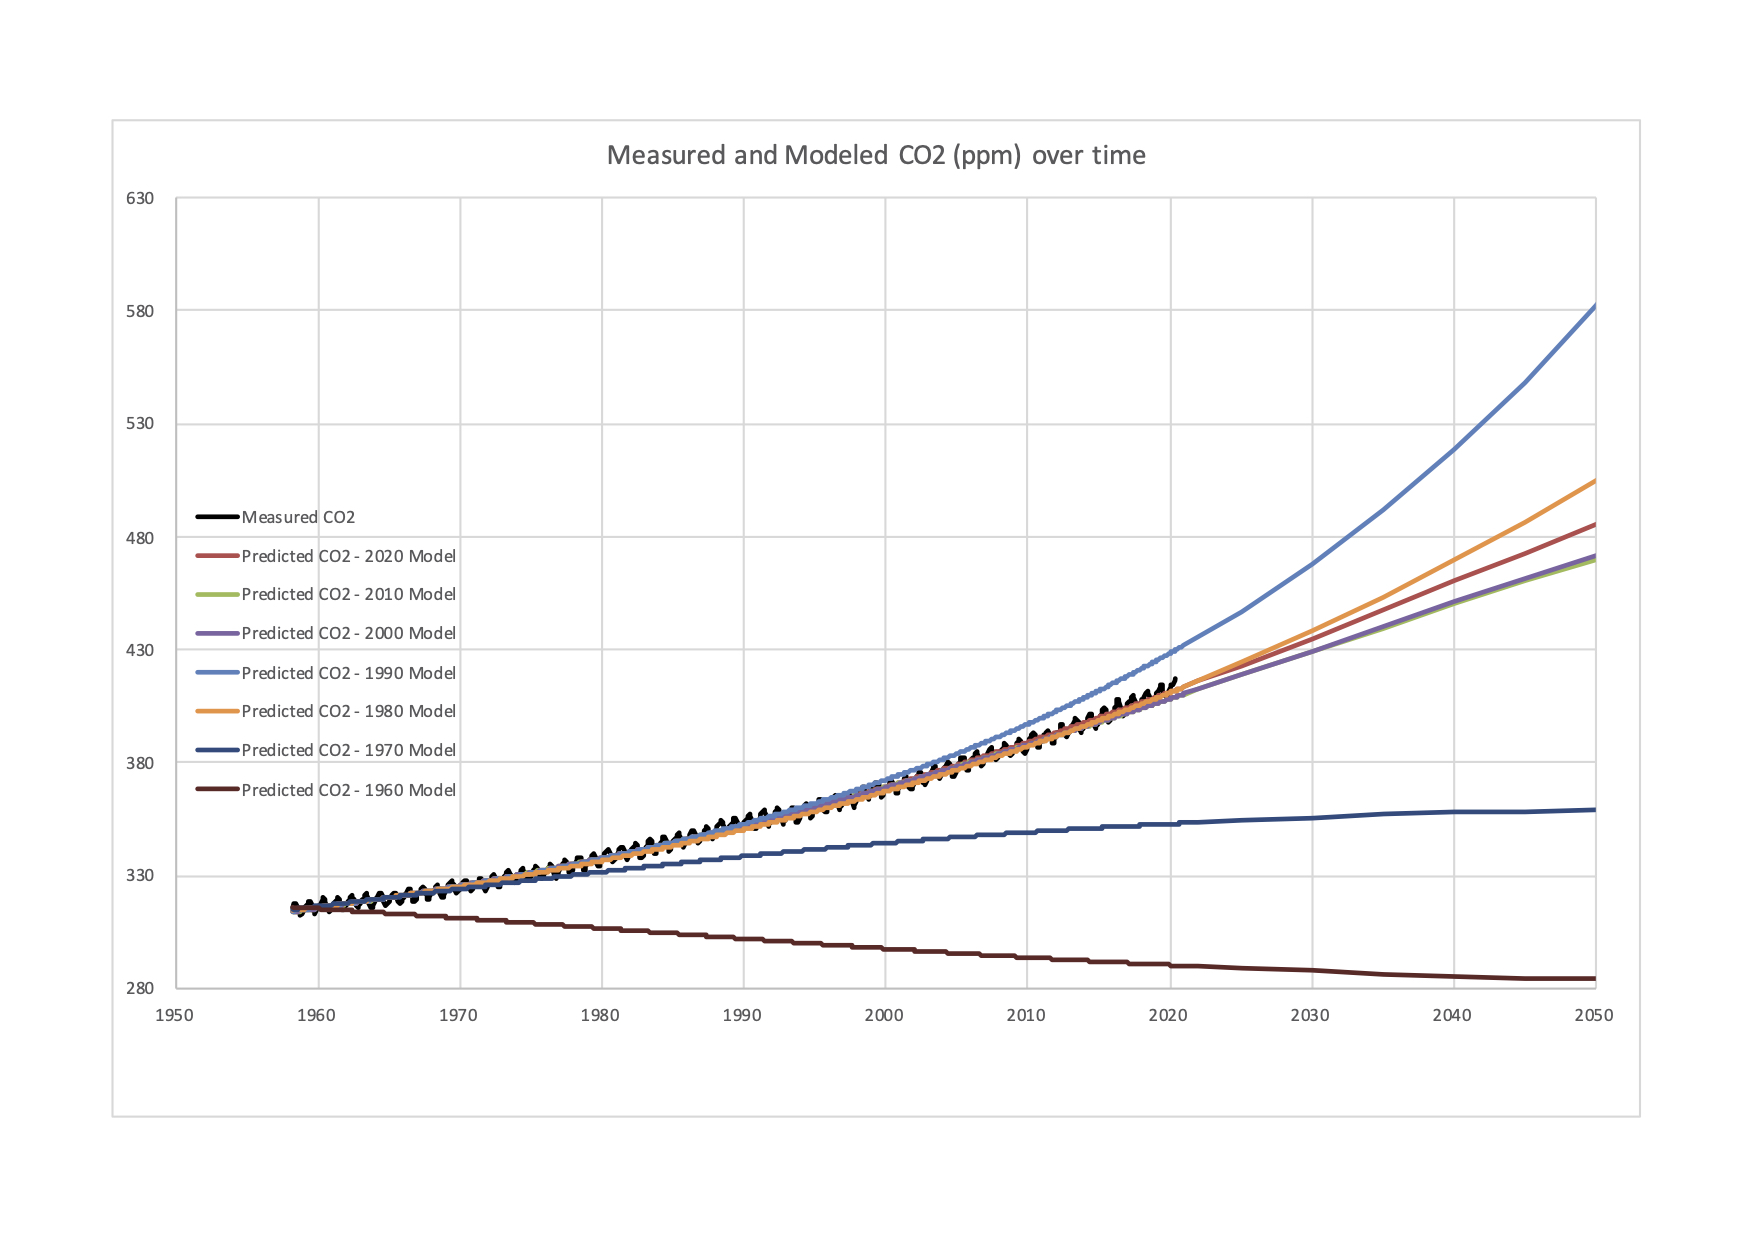
\includegraphics[width=\linewidth]{CO2-S-Curve.jpg}
\caption{Logistic Curves of $\mathrm{CO_{2}}$ Accumulation.}
\label{fig:results}
\end{figure}



\clearpage
\bibliographystyle{apacite}
\bibliography{bibliography}

\end{document}
